%\AtBeginDocument{%
\xsbox{fancybreakerbox}{%
  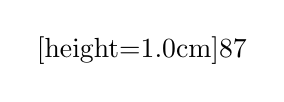
\begin{tikzpicture}
    \tikzset{pgfornamentstyle/.style={color=black,fill=stardustyellow, opacity=0.7, line width=0.5pt}}
    %\node[shift={(-3.5cm,0cm)},anchor=south east](L){\pgfornament[height=1cm]{79}};
    %\node[anchor=south]{\pgfornament[width=1.5cm]{9}};
    \node[anchor=south]{\pgfornament[height=1.0cm]{87}};
    %\node[shift={(+4cm,0cm)},anchor=south west](R){\pgfornament[symmetry=v,height=1cm]{79}};
    %\node[anchor=south]{\pgfornamenthline{L}{R}{south}{87}};
  \end{tikzpicture}
}
\newcommand{\fancybreaker}
